\chapter{Trajectory tracking via MPC}
 
\section{MPC Formulation and Implementation}
The goal of this task is to apply a Model Predictive Control (MPC) framework to track the optimal trajectory $(x^{\text{opt}}, u^{\text{opt}})$, which was generated in Task 2. The MPC ensures robustness to disturbances in the perturbed initial condition $x_0$.

For MPC computations, the dynamics of the system is approximated around the optimal trajectory generated in the Task 2, resulting in time-dependent matrices $A_t^{\text{opt}}$ and $B_t^{\text{opt}}$.
\begin{equation}
A_t^{\text{opt}} = \left.\frac{\partial f}{\partial x}\right|_{(x_t^{\text{opt}}, u_t^{\text{opt}})}, \quad
B_t^{\text{opt}} = \left.\frac{\partial f}{\partial u}\right|_{(x_t^{\text{opt}}, u_t^{\text{opt}})}
\end{equation}
The weighting matrices $Q_t$, $R_t$, and $Q_T$ are chosen to penalize deviations in states and inputs. All these matrices are positive definite, ensuring stability and good tracking performance.

At each time step $t$, the initial condition for the predicted trajectory is taken as the current measured state $x_t^{\text{meas}}$. 
\\
The optimization problem minimizes a cost function defined over the prediction horizon $T_{pred}$:

\[
\min_{\Delta x, \Delta u} \sum_{\tau=t}^{t+T-1} \left( \Delta x_\tau^\top Q_\tau \Delta x_\tau + \Delta u_\tau^\top R_\tau \Delta u_\tau \right) + \Delta x_{t+T}^\top Q_T \Delta x_{t+T}
\]

subject to:
\[
\begin{array}{l}
x_{\tau+1} = A_t^{\text{opt}}  x_\tau + B_t^{\text{opt}} \ u_\tau, \quad \quad \quad \tau = t, \dots, t+T-1 \\
x_\tau \in \mathcal{X}, \quad u_\tau \in \mathcal{U}, \quad \quad \quad \quad \quad \quad
\quad\tau = t, \dots, t+T \\
x_t^{\text{mpc}} = x_t^{\text{meas}}
\end{array}
\]

Here, $\Delta x = x_t^{\text{mpc}} - x_t^{\text{opt}}$ and $\Delta u = u_t^{\text{mpc}} - u_t^{\text{opt}}$ represent deviations from the optimal reference trajectory. 

The algorithm enforces specific constraints on the states and inputs to ensure safe and feasible operation:
\begin{equation}
u_{\text{min}} \leq u_\tau \leq u_{\text{max}}, \quad x_{\text{min}} \leq x_\tau \leq x_{\text{max}}, \quad \forall \tau \in [t, t+T]
\end{equation}
These constraints include limits on angular velocities, angles, and control inputs.

At each time step $t$, the algorithm solves the optimization problem to compute the predicted control inputs and state trajectories. However, only the first control input $u_t^{\text{mpc}}$ is applied to the system. At the next time step $t+1$, the state $x_{t+1}^{\text{meas}}$ is re-measured, and the optimization problem is solved again. This process allows the MPC to dynamically adapt the control actions, ensuring robustness to disturbances and modeling inaccuracies.


% - Linearize the dynamics around the generated trajectory.
% - Describe differences between MPC and LQR for tracking.
% - Discuss computational challenges and tuning parameters.

\section{Performance Analysis and Plots}
In Task 4, to test the tracking performance, a perturbed initial condition is considered, with a state perturbation percentage. In addition, the model accounts for both measurement and actuation noise to provide a more realistic representation of real-time implementation challenges.
\begin{table}[h!]
\centering
\begin{tabular}{|c|c|c|c|}
\hline
\textbf{Case} & \textbf{State Perturbation} & \textbf{Measurement Noise} & \textbf{Actuation Noise} \\ \hline
1        & 0.05                                   & 0                          & 0                          \\ \hline
2        & -0.1                                   & 0.005                      & 0.005                      \\ \hline
3        & -0.2                                   & 0.05                       & 0.05                       \\ \hline
\end{tabular}
\caption{State perturbation values, measurement noise, and attenuation noise for different cases}
\label{tab:perturbation_cases}
\end{table}

\begin{figure}[htb]
    \centering
    % First 3 images on the first page
    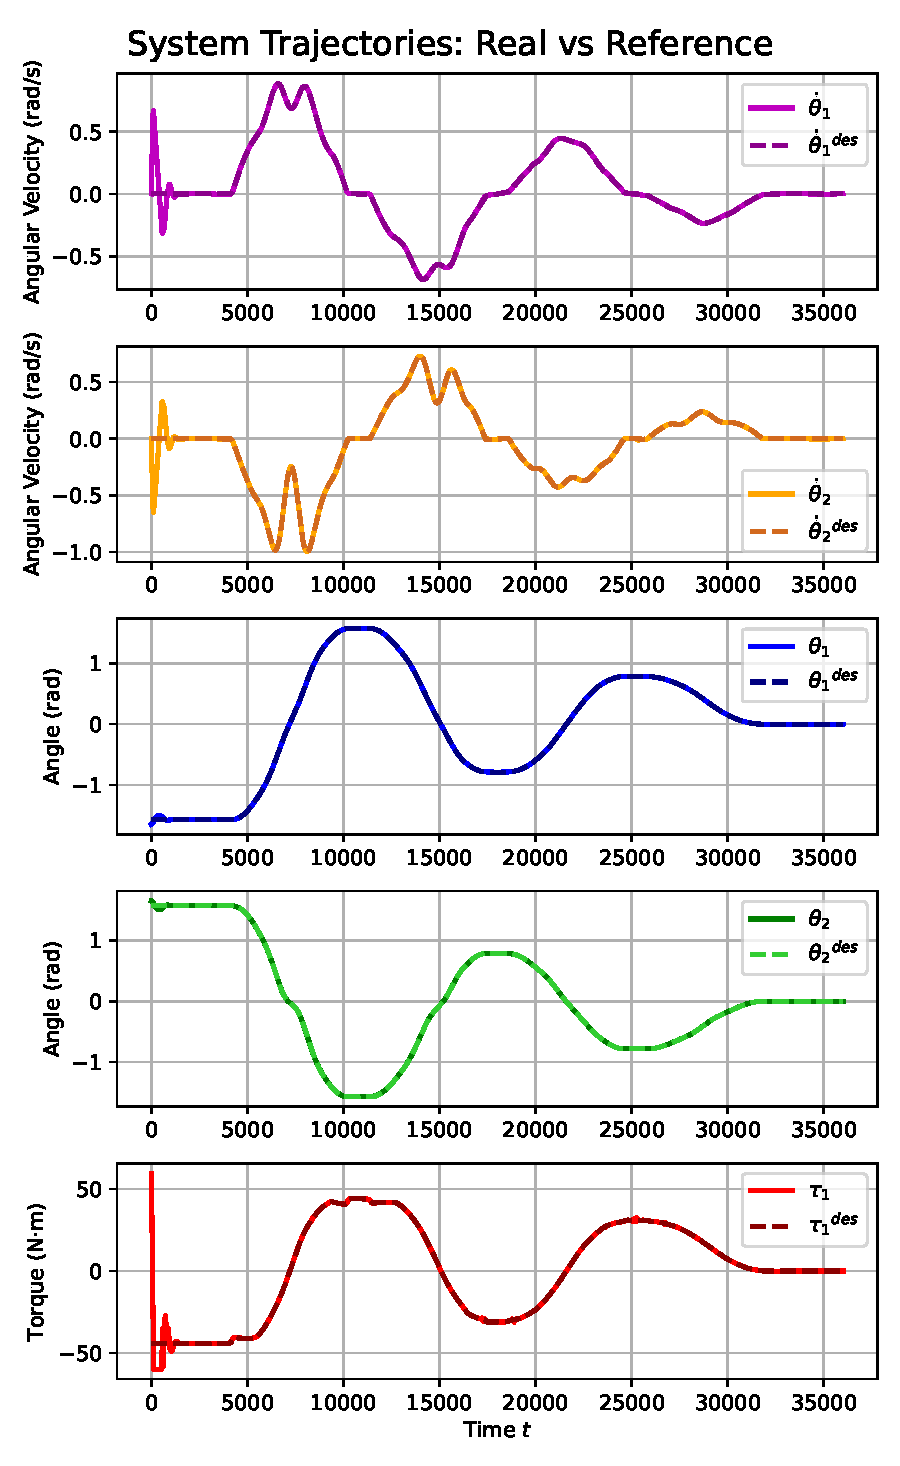
\includegraphics[width=1\linewidth]{img/4-task4/MPC1.pdf}
    \caption{Trajectories case 1}
    \label{fig:dtheta1-evolution}
\end{figure}

\begin{figure}[htb]
    \centering
    % First 3 images on the first page
    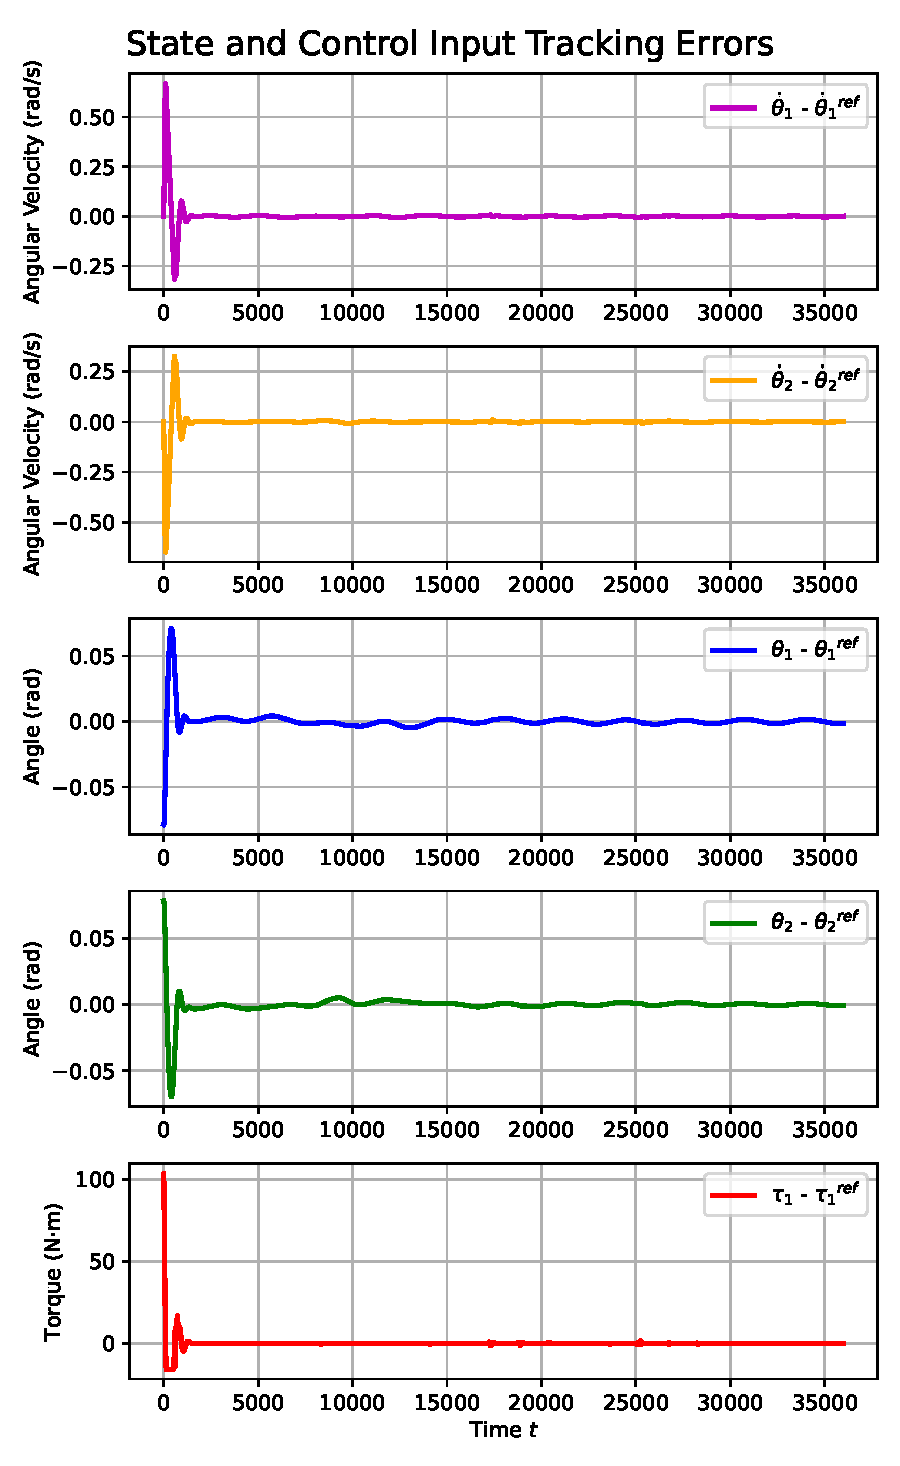
\includegraphics[width=1\linewidth]{img/4-task4/MPC1_errors.pdf}
    \caption{Tracking errors case 1}
    \label{fig:dtheta1-evolution}
\end{figure}

\begin{figure}[htb]
    \centering
    % First 3 images on the first page
    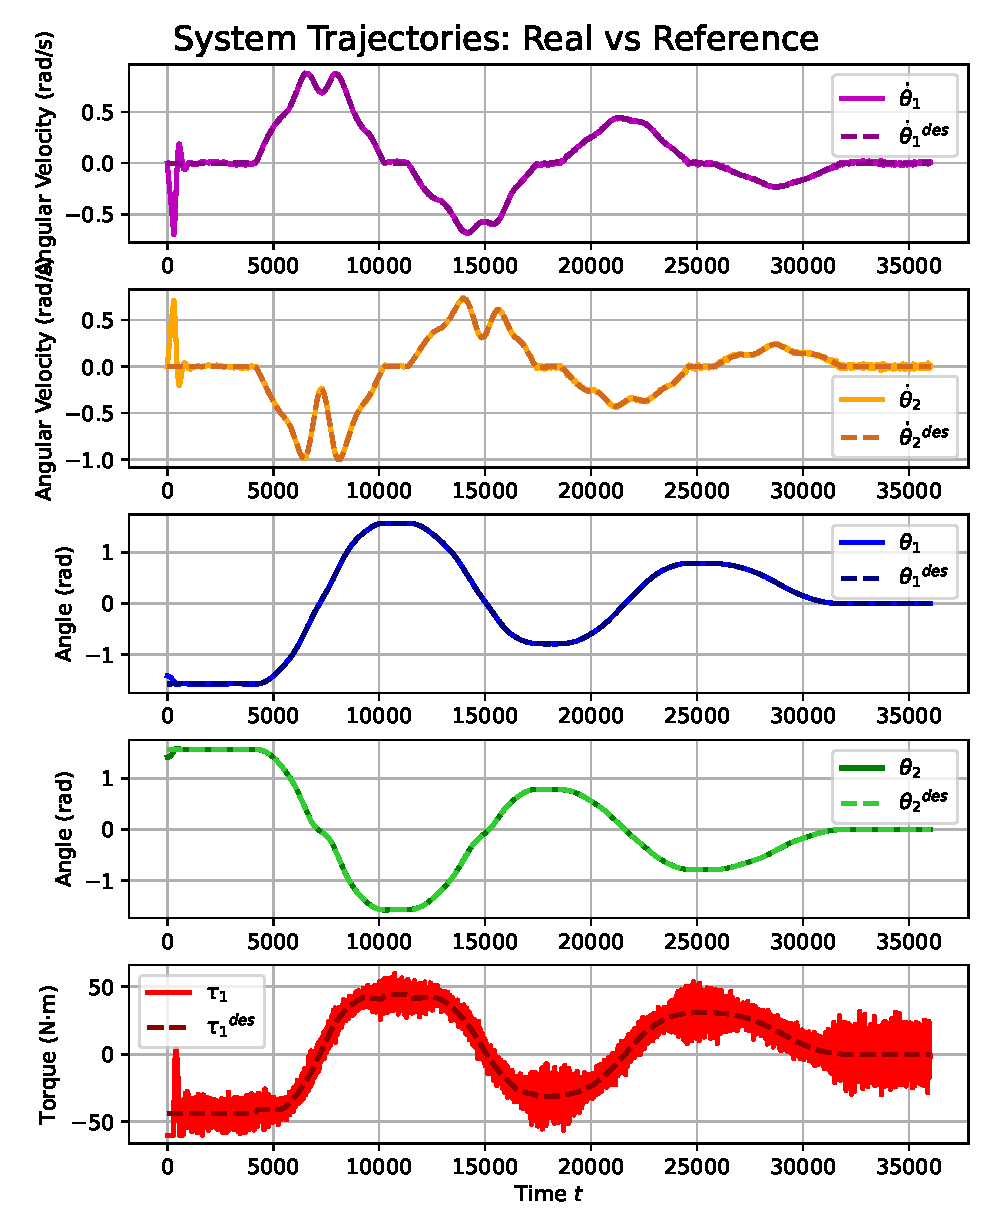
\includegraphics[width=1\linewidth]{img/4-task4/MPC2.pdf}
    \caption{Trajectories case 2}
    \label{fig:dtheta1-evolution}
\end{figure}

\begin{figure}[htb]
    \centering
    % First 3 images on the first page
    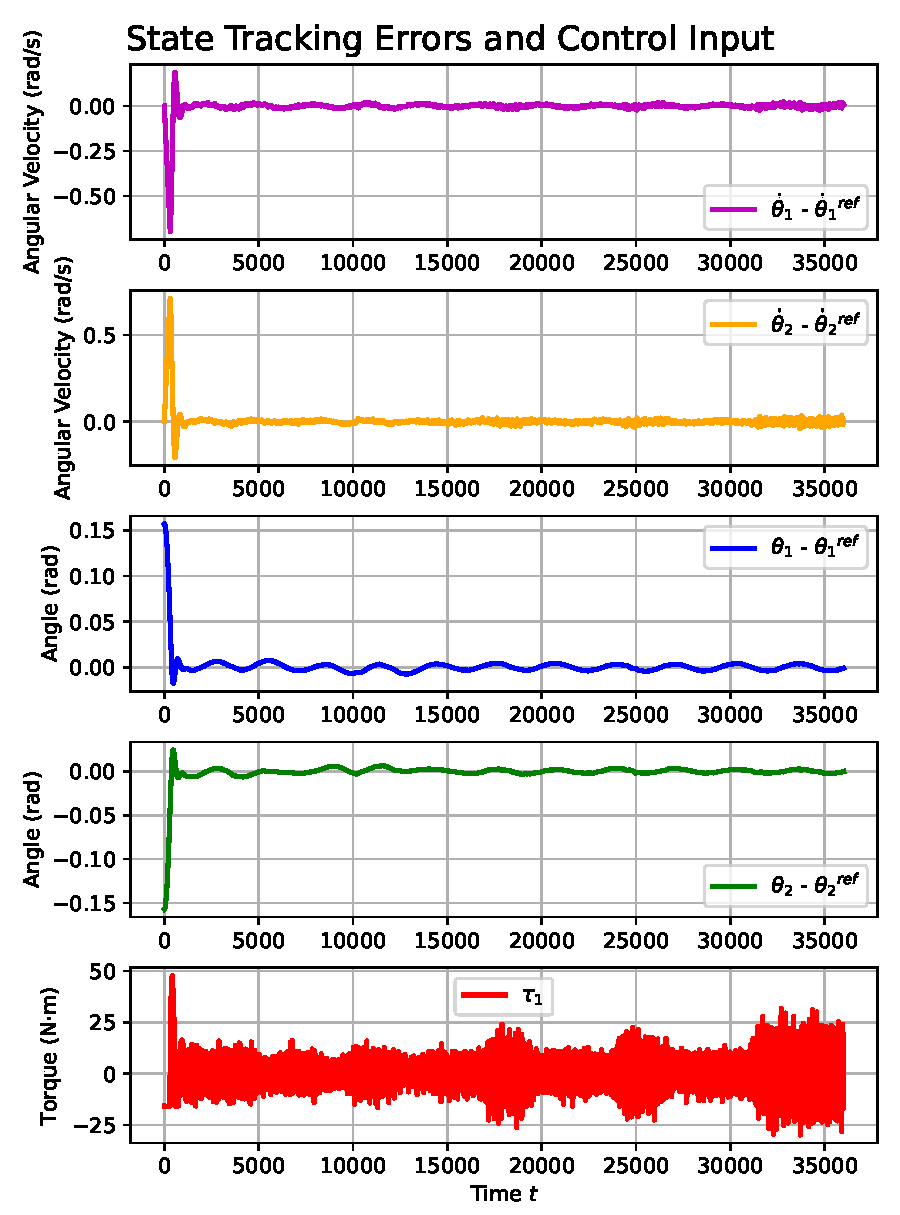
\includegraphics[width=1\linewidth]{img/4-task4/MPC2_errors.pdf}
    \caption{Tracking errors case 2}
    \label{fig:dtheta1-evolution}
\end{figure}

\begin{figure}[htb]
    \centering
    % First 3 images on the first page
    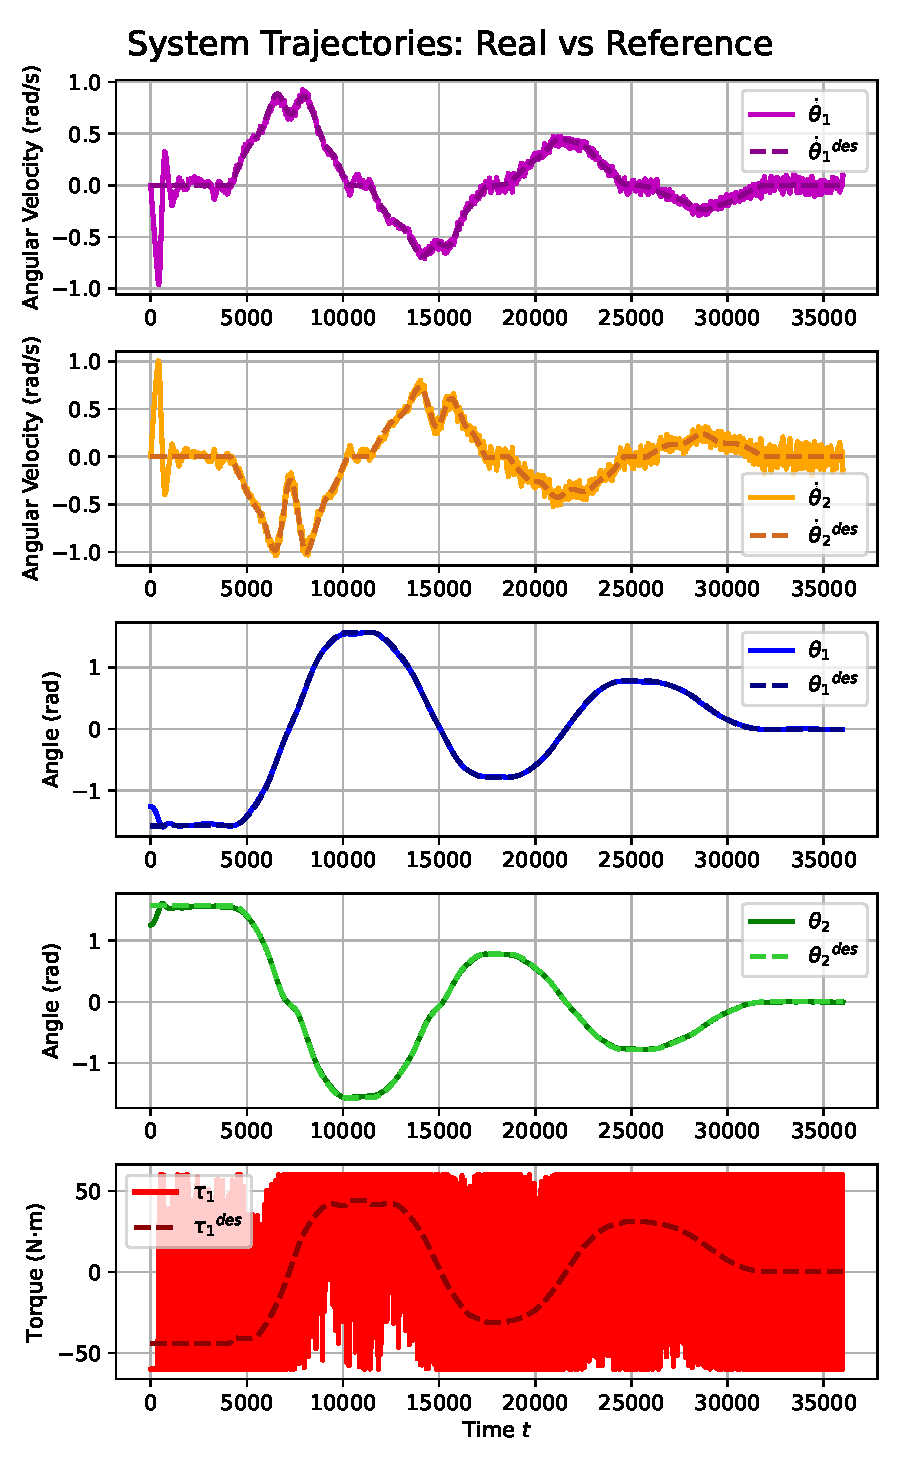
\includegraphics[width=1\linewidth]{img/4-task4/MPC3.pdf}
    \caption{Trajectories case 3}
    \label{fig:dtheta1-evolution}
\end{figure}

\begin{figure}[htb]
    \centering
    % First 3 images on the first page
    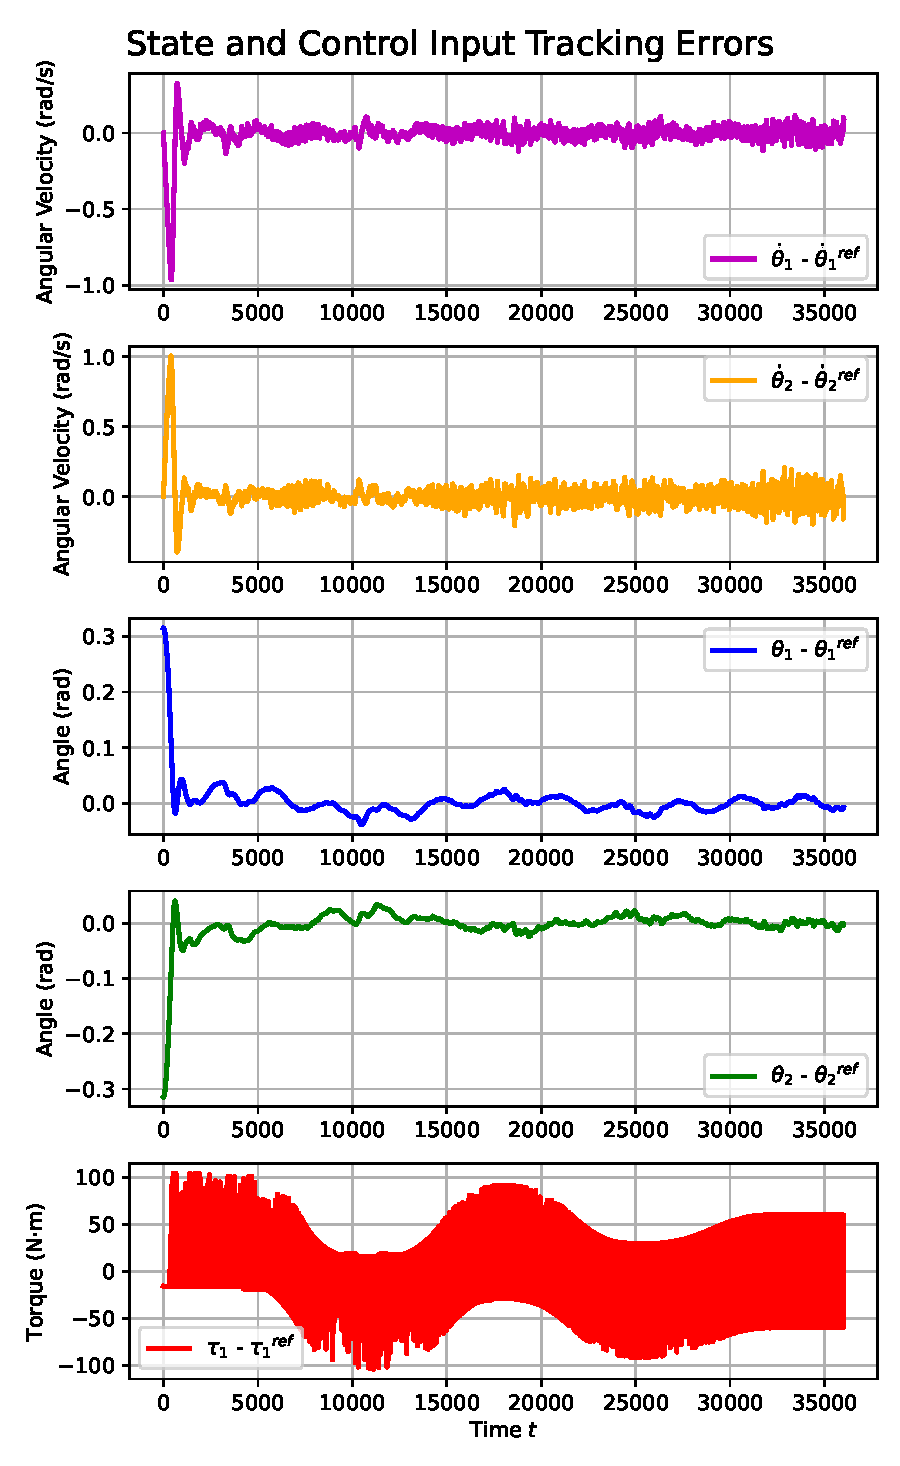
\includegraphics[width=1\linewidth]{img/4-task4/MPC3_errors.pdf}
    \caption{Tracking errors case 3}
    \label{fig:dtheta1-evolution}
\end{figure}
% - Required plots:
%   - System trajectory vs. desired trajectory.
%   - Tracking error under different initial conditions.
